% Options for packages loaded elsewhere
\PassOptionsToPackage{unicode}{hyperref}
\PassOptionsToPackage{hyphens}{url}
\PassOptionsToPackage{dvipsnames,svgnames,x11names}{xcolor}
%
\documentclass[
  letterpaper,
  DIV=11,
  numbers=noendperiod]{scrartcl}

\usepackage{amsmath,amssymb}
\usepackage{lmodern}
\usepackage{iftex}
\ifPDFTeX
  \usepackage[T1]{fontenc}
  \usepackage[utf8]{inputenc}
  \usepackage{textcomp} % provide euro and other symbols
\else % if luatex or xetex
  \usepackage{unicode-math}
  \defaultfontfeatures{Scale=MatchLowercase}
  \defaultfontfeatures[\rmfamily]{Ligatures=TeX,Scale=1}
\fi
% Use upquote if available, for straight quotes in verbatim environments
\IfFileExists{upquote.sty}{\usepackage{upquote}}{}
\IfFileExists{microtype.sty}{% use microtype if available
  \usepackage[]{microtype}
  \UseMicrotypeSet[protrusion]{basicmath} % disable protrusion for tt fonts
}{}
\makeatletter
\@ifundefined{KOMAClassName}{% if non-KOMA class
  \IfFileExists{parskip.sty}{%
    \usepackage{parskip}
  }{% else
    \setlength{\parindent}{0pt}
    \setlength{\parskip}{6pt plus 2pt minus 1pt}}
}{% if KOMA class
  \KOMAoptions{parskip=half}}
\makeatother
\usepackage{xcolor}
\setlength{\emergencystretch}{3em} % prevent overfull lines
\setcounter{secnumdepth}{-\maxdimen} % remove section numbering
% Make \paragraph and \subparagraph free-standing
\ifx\paragraph\undefined\else
  \let\oldparagraph\paragraph
  \renewcommand{\paragraph}[1]{\oldparagraph{#1}\mbox{}}
\fi
\ifx\subparagraph\undefined\else
  \let\oldsubparagraph\subparagraph
  \renewcommand{\subparagraph}[1]{\oldsubparagraph{#1}\mbox{}}
\fi

\usepackage{color}
\usepackage{fancyvrb}
\newcommand{\VerbBar}{|}
\newcommand{\VERB}{\Verb[commandchars=\\\{\}]}
\DefineVerbatimEnvironment{Highlighting}{Verbatim}{commandchars=\\\{\}}
% Add ',fontsize=\small' for more characters per line
\usepackage{framed}
\definecolor{shadecolor}{RGB}{241,243,245}
\newenvironment{Shaded}{\begin{snugshade}}{\end{snugshade}}
\newcommand{\AlertTok}[1]{\textcolor[rgb]{0.68,0.00,0.00}{#1}}
\newcommand{\AnnotationTok}[1]{\textcolor[rgb]{0.37,0.37,0.37}{#1}}
\newcommand{\AttributeTok}[1]{\textcolor[rgb]{0.40,0.45,0.13}{#1}}
\newcommand{\BaseNTok}[1]{\textcolor[rgb]{0.68,0.00,0.00}{#1}}
\newcommand{\BuiltInTok}[1]{\textcolor[rgb]{0.00,0.23,0.31}{#1}}
\newcommand{\CharTok}[1]{\textcolor[rgb]{0.13,0.47,0.30}{#1}}
\newcommand{\CommentTok}[1]{\textcolor[rgb]{0.37,0.37,0.37}{#1}}
\newcommand{\CommentVarTok}[1]{\textcolor[rgb]{0.37,0.37,0.37}{\textit{#1}}}
\newcommand{\ConstantTok}[1]{\textcolor[rgb]{0.56,0.35,0.01}{#1}}
\newcommand{\ControlFlowTok}[1]{\textcolor[rgb]{0.00,0.23,0.31}{#1}}
\newcommand{\DataTypeTok}[1]{\textcolor[rgb]{0.68,0.00,0.00}{#1}}
\newcommand{\DecValTok}[1]{\textcolor[rgb]{0.68,0.00,0.00}{#1}}
\newcommand{\DocumentationTok}[1]{\textcolor[rgb]{0.37,0.37,0.37}{\textit{#1}}}
\newcommand{\ErrorTok}[1]{\textcolor[rgb]{0.68,0.00,0.00}{#1}}
\newcommand{\ExtensionTok}[1]{\textcolor[rgb]{0.00,0.23,0.31}{#1}}
\newcommand{\FloatTok}[1]{\textcolor[rgb]{0.68,0.00,0.00}{#1}}
\newcommand{\FunctionTok}[1]{\textcolor[rgb]{0.28,0.35,0.67}{#1}}
\newcommand{\ImportTok}[1]{\textcolor[rgb]{0.00,0.46,0.62}{#1}}
\newcommand{\InformationTok}[1]{\textcolor[rgb]{0.37,0.37,0.37}{#1}}
\newcommand{\KeywordTok}[1]{\textcolor[rgb]{0.00,0.23,0.31}{#1}}
\newcommand{\NormalTok}[1]{\textcolor[rgb]{0.00,0.23,0.31}{#1}}
\newcommand{\OperatorTok}[1]{\textcolor[rgb]{0.37,0.37,0.37}{#1}}
\newcommand{\OtherTok}[1]{\textcolor[rgb]{0.00,0.23,0.31}{#1}}
\newcommand{\PreprocessorTok}[1]{\textcolor[rgb]{0.68,0.00,0.00}{#1}}
\newcommand{\RegionMarkerTok}[1]{\textcolor[rgb]{0.00,0.23,0.31}{#1}}
\newcommand{\SpecialCharTok}[1]{\textcolor[rgb]{0.37,0.37,0.37}{#1}}
\newcommand{\SpecialStringTok}[1]{\textcolor[rgb]{0.13,0.47,0.30}{#1}}
\newcommand{\StringTok}[1]{\textcolor[rgb]{0.13,0.47,0.30}{#1}}
\newcommand{\VariableTok}[1]{\textcolor[rgb]{0.07,0.07,0.07}{#1}}
\newcommand{\VerbatimStringTok}[1]{\textcolor[rgb]{0.13,0.47,0.30}{#1}}
\newcommand{\WarningTok}[1]{\textcolor[rgb]{0.37,0.37,0.37}{\textit{#1}}}

\providecommand{\tightlist}{%
  \setlength{\itemsep}{0pt}\setlength{\parskip}{0pt}}\usepackage{longtable,booktabs,array}
\usepackage{calc} % for calculating minipage widths
% Correct order of tables after \paragraph or \subparagraph
\usepackage{etoolbox}
\makeatletter
\patchcmd\longtable{\par}{\if@noskipsec\mbox{}\fi\par}{}{}
\makeatother
% Allow footnotes in longtable head/foot
\IfFileExists{footnotehyper.sty}{\usepackage{footnotehyper}}{\usepackage{footnote}}
\makesavenoteenv{longtable}
\usepackage{graphicx}
\makeatletter
\def\maxwidth{\ifdim\Gin@nat@width>\linewidth\linewidth\else\Gin@nat@width\fi}
\def\maxheight{\ifdim\Gin@nat@height>\textheight\textheight\else\Gin@nat@height\fi}
\makeatother
% Scale images if necessary, so that they will not overflow the page
% margins by default, and it is still possible to overwrite the defaults
% using explicit options in \includegraphics[width, height, ...]{}
\setkeys{Gin}{width=\maxwidth,height=\maxheight,keepaspectratio}
% Set default figure placement to htbp
\makeatletter
\def\fps@figure{htbp}
\makeatother

\KOMAoption{captions}{tableheading}
\makeatletter
\makeatother
\makeatletter
\makeatother
\makeatletter
\@ifpackageloaded{caption}{}{\usepackage{caption}}
\AtBeginDocument{%
\ifdefined\contentsname
  \renewcommand*\contentsname{Table of contents}
\else
  \newcommand\contentsname{Table of contents}
\fi
\ifdefined\listfigurename
  \renewcommand*\listfigurename{List of Figures}
\else
  \newcommand\listfigurename{List of Figures}
\fi
\ifdefined\listtablename
  \renewcommand*\listtablename{List of Tables}
\else
  \newcommand\listtablename{List of Tables}
\fi
\ifdefined\figurename
  \renewcommand*\figurename{Figure}
\else
  \newcommand\figurename{Figure}
\fi
\ifdefined\tablename
  \renewcommand*\tablename{Table}
\else
  \newcommand\tablename{Table}
\fi
}
\@ifpackageloaded{float}{}{\usepackage{float}}
\floatstyle{ruled}
\@ifundefined{c@chapter}{\newfloat{codelisting}{h}{lop}}{\newfloat{codelisting}{h}{lop}[chapter]}
\floatname{codelisting}{Listing}
\newcommand*\listoflistings{\listof{codelisting}{List of Listings}}
\makeatother
\makeatletter
\@ifpackageloaded{caption}{}{\usepackage{caption}}
\@ifpackageloaded{subcaption}{}{\usepackage{subcaption}}
\makeatother
\makeatletter
\@ifpackageloaded{tcolorbox}{}{\usepackage[many]{tcolorbox}}
\makeatother
\makeatletter
\@ifundefined{shadecolor}{\definecolor{shadecolor}{rgb}{.97, .97, .97}}
\makeatother
\makeatletter
\makeatother
\ifLuaTeX
  \usepackage{selnolig}  % disable illegal ligatures
\fi
\IfFileExists{bookmark.sty}{\usepackage{bookmark}}{\usepackage{hyperref}}
\IfFileExists{xurl.sty}{\usepackage{xurl}}{} % add URL line breaks if available
\urlstyle{same} % disable monospaced font for URLs
\hypersetup{
  pdftitle={Better Call Sauls Series},
  pdfauthor={Dawid Szyszko-Celinski},
  colorlinks=true,
  linkcolor={blue},
  filecolor={Maroon},
  citecolor={Blue},
  urlcolor={Blue},
  pdfcreator={LaTeX via pandoc}}

\title{Better Call Sauls Series}
\author{Dawid Szyszko-Celinski}
\date{5/18/23}

\begin{document}
\maketitle
\ifdefined\Shaded\renewenvironment{Shaded}{\begin{tcolorbox}[frame hidden, borderline west={3pt}{0pt}{shadecolor}, breakable, boxrule=0pt, enhanced, interior hidden, sharp corners]}{\end{tcolorbox}}\fi

\begin{center}\rule{0.5\linewidth}{0.5pt}\end{center}

\hypertarget{description}{%
\subsection{Description}\label{description}}

Better Call Saul is an American legal crime drama television series
created by \emph{Vince Gilligan} and \emph{Peter Gould} for AMC. Part of
the Breaking Bad franchise, it is a spin-off from Gilligan's previous
series, Breaking Bad, to which it serves as both a prequel and sequel.
Better Call Saul premiered on AMC on February 8, 2015, and concluded on
August 15, 2022, after six seasons consisting of 63 episodes.

Set primarily in the early 2000s in Albuquerque, New Mexico, several
years before Breaking Bad, Better Call Saul examines the moral declines
of \emph{Jimmy McGill (Bob Odenkirk)}, an earnest lawyer and former con
artist who becomes the egocentric criminal-defense attorney \emph{Saul
Goodman}, and \emph{Mike Ehrmantraut (Jonathan Banks)}, a former police
officer who becomes a fixer and enforcer for drug traffickers. Other
main characters include Jimmy's romantic interest and colleague
\emph{Kim Wexler (Rhea Seehorn)}, his brother and rival \emph{Chuck
McGill (Michael McKean)}, Chuck's law partner \emph{Howard Hamlin
(Patrick Fabian)}, the drug dealer \emph{Nacho Varga (Michael Mando)},
the drug lord \emph{Gus Fring (Giancarlo Esposito)}, and the cartel
enforcer \emph{Lalo Salamanca (Tony Dalton)}. In addition to the primary
storyline, Better Call Saul includes black-and-white flashforwards set
in 2010, after the events of Breaking Bad, which explore the
consequences of Saul's eventual partnership with the drug lord
\emph{Walter White (Bryan Cranston)}.

\hypertarget{photo}{%
\subsection{2 Photo}\label{photo}}

\hypertarget{statistics}{%
\subsection{3 Statistics}\label{statistics}}

\begin{Shaded}
\begin{Highlighting}[]
\InformationTok{\textasciigrave{}\textasciigrave{}\textasciigrave{}\{r\}}
\NormalTok{stats }\OtherTok{\textless{}{-}} \FunctionTok{data.frame}\NormalTok{(}\AttributeTok{season =} \FunctionTok{c}\NormalTok{(}\DecValTok{1}\NormalTok{,}\DecValTok{2}\NormalTok{,}\DecValTok{3}\NormalTok{,}\DecValTok{4}\NormalTok{,}\DecValTok{5}\NormalTok{,}\DecValTok{6}\NormalTok{), }\AttributeTok{avg.view =} \FunctionTok{c}\NormalTok{(}\FloatTok{3.21}\NormalTok{,}\FloatTok{2.16}\NormalTok{,}\FloatTok{1.64}\NormalTok{,}\FloatTok{1.49}\NormalTok{,}\FloatTok{1.37}\NormalTok{,}\FloatTok{1.27}\NormalTok{))}
\FunctionTok{summary}\NormalTok{(stats)}
\InformationTok{\textasciigrave{}\textasciigrave{}\textasciigrave{}}
\end{Highlighting}
\end{Shaded}

\begin{verbatim}
     season        avg.view    
 Min.   :1.00   Min.   :1.270  
 1st Qu.:2.25   1st Qu.:1.400  
 Median :3.50   Median :1.565  
 Mean   :3.50   Mean   :1.857  
 3rd Qu.:4.75   3rd Qu.:2.030  
 Max.   :6.00   Max.   :3.210  
\end{verbatim}

\hypertarget{graph}{%
\subsection{4 Graph}\label{graph}}

\begin{Shaded}
\begin{Highlighting}[]
\InformationTok{\textasciigrave{}\textasciigrave{}\textasciigrave{}\{r\}}
\FunctionTok{plot}\NormalTok{(stats)}
\InformationTok{\textasciigrave{}\textasciigrave{}\textasciigrave{}}
\end{Highlighting}
\end{Shaded}

\begin{figure}[H]

{\centering 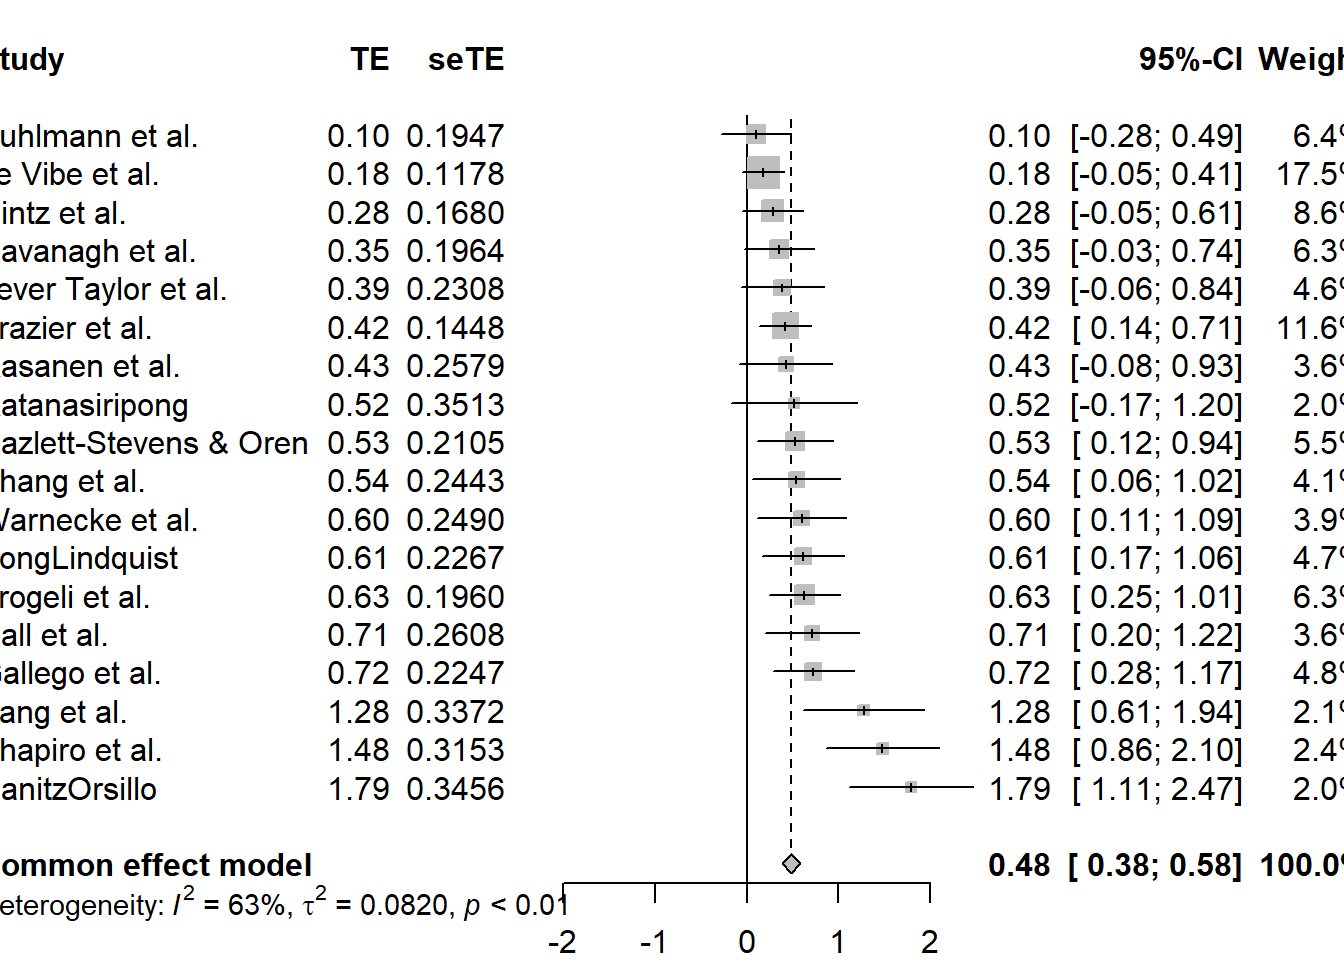
\includegraphics{Assignment_DSC2_files/figure-pdf/unnamed-chunk-6-1.pdf}

}

\end{figure}

\hypertarget{decrease}{%
\subsection{6 Decrease}\label{decrease}}

\begin{Shaded}
\begin{Highlighting}[]
\InformationTok{\textasciigrave{}\textasciigrave{}\textasciigrave{}\{r\}}
\NormalTok{views1 }\OtherTok{\textless{}{-}} \FloatTok{3.21}
\NormalTok{views3 }\OtherTok{\textless{}{-}} \FloatTok{1.64}
\NormalTok{diff }\OtherTok{\textless{}{-}}\NormalTok{ views1 }\SpecialCharTok{{-}}\NormalTok{ views3}
\InformationTok{\textasciigrave{}\textasciigrave{}\textasciigrave{}}
\end{Highlighting}
\end{Shaded}

In a first season there were 3.21 M views on average, on season three
1.64 M views on average and difference between seasons 1.57 M views.

\hypertarget{section}{%
\subsection{7}\label{section}}

\hypertarget{assignment}{%
\section{ASSIGNMENT}\label{assignment}}

\hypertarget{lists}{%
\section{Lists}\label{lists}}

\hypertarget{ordered}{%
\paragraph{Ordered}\label{ordered}}

\texttt{1.\ Item\ 1}

\texttt{2.\ Item\ 2}

\texttt{2.\ Item\ 3\ \#\ Note\ the\ error\ in\ numbering}

\begin{enumerate}
\def\labelenumi{\arabic{enumi}.}
\item
  Item 1
\item
  Item 2
\item
  Item 3 \texttt{\#\ It\textquotesingle{}s\ fine\ here\ though}
\end{enumerate}

\hypertarget{unordered}{%
\paragraph{Unordered}\label{unordered}}

\texttt{*\ Item}

\texttt{*\ Another\ item}

\begin{itemize}
\item
  Item
\item
  Another item
\end{itemize}

\hypertarget{subitems}{%
\paragraph{Subitems}\label{subitems}}

\texttt{1.\ \ Item\ 1}

\texttt{-\ \ \ Item\ 2}

\texttt{-\ \ \ Item\ 3}

\begin{enumerate}
\def\labelenumi{\arabic{enumi}.}
\tightlist
\item
  Item 1

  \begin{itemize}
  \tightlist
  \item
    Item 2
  \item
    Item 3
  \end{itemize}
\end{enumerate}

Pick a TV show that had its premieres on TV and thus has some viewership
numbers reported on Wikipedia. E.g.
\href{https://en.wikipedia.org/wiki/List_of_Suits_episodes}{Suits} (see
table just above the References)

Then create a short report (you can copy the content from Wikipedia or
other pages for this task) that contains, for example:

(do a commit after each step!)

\begin{enumerate}
\def\labelenumi{\arabic{enumi}.}
\tightlist
\item
  A brief description of the show (use \emph{italics} for names).
\item
  A photo with the logo or a shot from the show itself.
\item
  A summary of some basic statistics (e.g.~on viewership or ratings).
\item
  A graph of the viewership over time.
\item
  A graph of the episode-to-episode (or season-to-season) changes in
  viewership.
\item
  A short description of the observed changes that includes inline
  references to numbers (e.g.~the viewership decreased by
  \texttt{insert\_calculated\_number} between seasons 3 and 5).
\item
  Make sure your report looks nice -\textgreater{} this time we're
  mostly interested in the output and not necessarily the codes used to
  achieve it.
\item
  \texttt{render} your report and save it in the relevant folder of your
  repo.
\item
  Commit the changes and push them to Github.
\end{enumerate}



\end{document}
